\chapter{Примеры задач аппроксимации статистических данных}

\paragraph*{Пример 1~\cite{markov24}}
В таблице~\ref{tbl:example1} приведены данные о растворимости
азотнокислого натрия \( NaNO_3 \) в 100 частях воды зависимости от её температуры.

\begin{table}[h!]
  \caption{Данные о растворимости \( NaNO_3 \) в зависимости от температуры воды\label{tbl:example1}}
  \small
  \begin{tabular}{| m{5.5cm} | c | c | c | c | c | c | c | c | c |}
    \hline
    Температура воды, °С
    & 0
    & 4
    & 10
    & 15
    & 21
    & 29
    & 36
    & 51
    & 68 \\
    \hline
    Число условных \par
    частей растворенного \par
    \( NaNO_3 \)
    & 66{,}7
    & 71{,}0
    & 76{,}3
    & 80{,}6
    & 85{,}7
    & 92{,}9
    & 99{,}4
    & 113{,}6
    & 125{,}1 \\
    \hline
    \end{tabular}
\end{table}

Теоретические соображения позволяют думать,
что количественная сторона этого явления довольно точно описывается линейной зависимостью
\begin{equation}
  \label{eq:example1}
  y = a + bx,
\end{equation}
где
\( x \) --- температура в градусах, а
\( y \) --- растворимость в условных частях на 100 частей воды.

Требуется на основании данных~\ref{tbl:example1} определить оценки параметров
\( \hat{x}, \hat{y} \) соотношения~\eqref{eq:example1}.

\paragraph*{Пример 2~\cite{ezekiel41}}

Производится наблюдение над двумя переменными ---
процентным содержанием протеина \( x \) и крахмала \( у \) в зернах пшеницы.
Обе переменные характеризуют качество пшеницы, но определение \( х \) требует
сложного химического анализа, а определение \( у \) может быть сделано
гораздо проще и без приборов.
В таблице~\ref{tbl:example2} приведены результаты 20 наблюдений.

Требуется на основании данных~\ref{tbl:example2} определить оценки параметров
\( \hat{a}, \hat{b}, \hat{c} \) параметров соотношения~\eqref{eq:example2}.
\begin{equation}
  \label{eq:example2}
  y = a + bx + cx^2.
\end{equation}

\begin{table}[ht]
  \caption{Данные о содержании протеина и крахмала в зернах пшеницы\label{tbl:example2}}
  \small
  \begin{tabular}{| m{4.8cm} | c | c | c | c | c | c | c | c | c | c |}
    \hline
    \textnumero~наблюдения
    & 1
    & 2
    & 3
    & 4
    & 5
    & 6
    & 7
    & 8
    & 9
    & 10 \\
    \hline
    Содержание протеина, \%
    & 10{,}3
    & 12{,}2
    & 14{,}5
    & 11{,}1
    & 10{,}9
    & 18{,}1
    & 14{,}0
    & 10{,}8
    & 11{,}4
    & 11{,}0 \\
    \hline
    Содержание крахмала, \%
    & 6
    & 75
    & 87
    & 55
    & 34
    & 98
    & 91
    & 45
    & 51
    & 17 \\
    \hline
    \hline
    \textnumero~наблюдения
    & 1
    & 2
    & 3
    & 4
    & 5
    & 6
    & 7
    & 8
    & 9
    & 10 \\
    \hline
    Содержание протеина, \%
    & 10{,}2
    & 17{,}0
    & 13{,}8
    & 10{,}1
    & 14{,}4
    & 15{,}8
    & 15{,}6
    & 15{,}0
    & 13{,}3
    & 19{,}0 \\
    \hline
    Содержание крахмала, \%
    & 36
    & 97
    & 74
    & 24
    & 85
    & 96
    & 92
    & 94
    & 84
    & 99 \\
    \hline
    \end{tabular}
\end{table}

\paragraph*{Пример 3~\cite{linnik62}}

При математико-статистическом описании неровностей профиля поверхности при
производственной обработке важную роль играет понятие средней линии случайного профиля.
В весьма упрощенной форме задачу нахождения средней линии профиля можно поставить следующим образом.
На плоскости \( XOY \), представленной на рисунке~\ref{fig:example3},
задан ряд точек \( (x_i, y_i), i = 1, 2, \ldots \).
Требуется провести прямую \( y = ax + b \) так,
чтобы сумма квадратов расстояний точек \( (x_i, у_i) \) от этой прямой была минимальной.

\begin{figure}[h!]
  \centering
  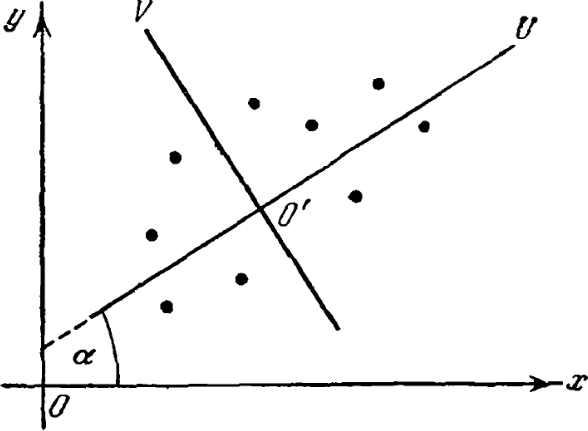
\includegraphics[width=92mm]{fig/example3}
  \caption{Средняя линия профиля}\label{fig:example3}
\end{figure}

С механической точки зрения прямая \( U \) представляет собой ось вращения,
дающую данной системе точек наименьший момент инерции
(наименьшую кинетическую энергию вращения при заданной угловой скорости).
Такая ось проходит через центр тяжести системы, а перпендикулярная ей ось \( V \),
проходящая через центр тяжести, будет давать для той же системы максимальный момент инерции.

\pagebreak
\paragraph*{Пример 4~\cite{kruchkova02}}

Фирмы часто испытывают необходимость в проектировании и освоении производства такой продукции,
которая не заменяет ранее освоенную, а дополняет или расширяет уже существующий параметрический ряд
изделий. Под параметрическим рядом понимается совокупность конструктивно и
технологически однородных изделий, предназначенных для выполнения одних и тех же функций и
отличающихся друг от друга значениями технико-экономических параметров в соответствии с
выполняемыми производственными операциями.
Анализ производственных затрат позволяет установить, что нормы расхода материальных ресурсов,
как правило, изменяются при корректировке технико-экономических параметров.

Для определения цены такой продукции необходимо определить зависимость изменения цены от
изменения технико-экономических параметров относящейся к данному ряду
\begin{equation}
  \label{eq:example4}
  P = f(X_1, X_2, \ldots, X_n),
\end{equation}
где \( X_1, X_2, \ldots, X_n \) --- параметры изделия.
Цена нового изделия рассчитывается путем подстановки значений его параметров в~\eqref{eq:example4}.

\paragraph*{Пример 5}

Еще одной задачей аппроксимации статистических данных является задача
определения связи итогов голосования за власть \( Y \) с показателями \( x_1, \ldots x_n \),
учитывающими уровень экономического развития региона:
\begin{equation}
  Y = c_0 + \sum_{i=1}^n c_i x_i,
\end{equation}
где \( c_1, \ldots, c_n \) --- параметры модели.

В работе~\cite{mau98} на основе данных о федеральных выборах в Государственную Думу РФ
(декабрь 1995) и президентских выборах РФ (июнь 1996) было показано, что
чем лучше по сравнению с другими субъектами Российской Федерации развит регион,
тем больше население поддерживает существующую власть.
